\subsection{Parametry początkowe używane do badania wpływu parametrów}

\begin{table}[htbp]
\centering
\caption{Parametry początkowe algorytmu}
\label{tab:params}
\begin{tabular}{|c|c|}
\hline
Parametr & Wartość \\
\hline
Rozmiar populacji & 400 \\
Maksymalna liczba generacji & 1500 \\
Wymiar & 20 \\
Minimalna częstotliwość & 0 \\
Maksymalna częstotliwość & 1 \\
Alpha & 0.5 \\
Epsilon & 0.5 \\
Alpha levy & 1.5 \\
\hline
\end{tabular}
\end{table}

\subsection{Dobór parametrów}

W tej sekcji badaniu poddane zostaną parametry wejściowe obu algorytmów oraz ich wpływ na ostateczny wynik, w tym celu posłużymy się manipulacjami na funkcji Rastring, jej wolny spadek pozwoli dokładniej zobrazować wpływ wprowadzonych zmian.

\subsection{Wpływ rozmiaru populacji dla algorytmu nietoperza}

\begin{figure}[H]
\centering
\includegraphics[width=1\textwidth]{plots/bat_population.png}
\caption{Wynik eksperymentu dla populacji dla algorytmu nietoperza.}
\label{fig:population_bat}
\end{figure}

\subsection{Wpływ populacji dla algorytmu BOA z lotem Levy’ego}

\begin{figure}[H]
\centering
\includegraphics[width=1\textwidth]{plots/boa_levy_population.png}
\caption{Wynik eksperymentu dla populacji dla algorytmu BOA z lotem Levy’ego.}
\label{fig:population_levy}
\end{figure}

\subsection{Wpływ liczby iteracji dla algorytmu nietoperza}

\begin{figure}[H]
\centering
\includegraphics[width=1\textwidth]{plots/bat_iterations.png}
\caption{Wynik eksperymentu dla liczby iteracji dla algorytmu nietoperza.}
\label{fig:iterations_bat}
\end{figure}

\subsection{Wpływ liczby iteracji dla algorytmu BOA z lotem Levy’ego}

\begin{figure}[H]
\centering
\includegraphics[width=1\textwidth]{plots/boa_levy_iterations.png}
\caption{Wynik eksperymentu dla liczby iteracji dla algorytmu BOA z lotem Levy’ego.}
\label{fig:iterations_levy}
\end{figure}

\subsection{Wpływ wymiarów dla algorytmu nietoperza}

\begin{figure}[H]
\centering
\includegraphics[width=1\textwidth]{plots/bat_dimensions.png}
\caption{Wynik eksperymentu dla wymiarów dla algorytmu nietoperza.}
\label{fig:dimensions_bat}
\end{figure}

\subsection{Wpływ wymiarów dla algorytmu BOA z lotem Levy’ego}

\begin{figure}[H]
\centering
\includegraphics[width=1\textwidth]{plots/boa_levy_dimensions.png}
\caption{Wynik eksperymentu dla wymiarów dla algorytmu BOA z lotem Levy’ego.}
\label{fig:dimensions_levy}
\end{figure}

\subsection{Wpływ parametru Maksymalnej częstotliwości dla algorytmu nietoperza}

\begin{figure}[H]
\centering
\includegraphics[width=1\textwidth]{plots/bat_frequency.png}
\caption{Wynik eksperymentu dla parametru Maksymalnej częstotliwości dla algorytmu nietoperza.}
\label{fig:frequency_bat}
\end{figure}

\subsection{Wpływ parametru $\alpha$ dla algorytmu nietoperza}

\begin{figure}[H]
\centering
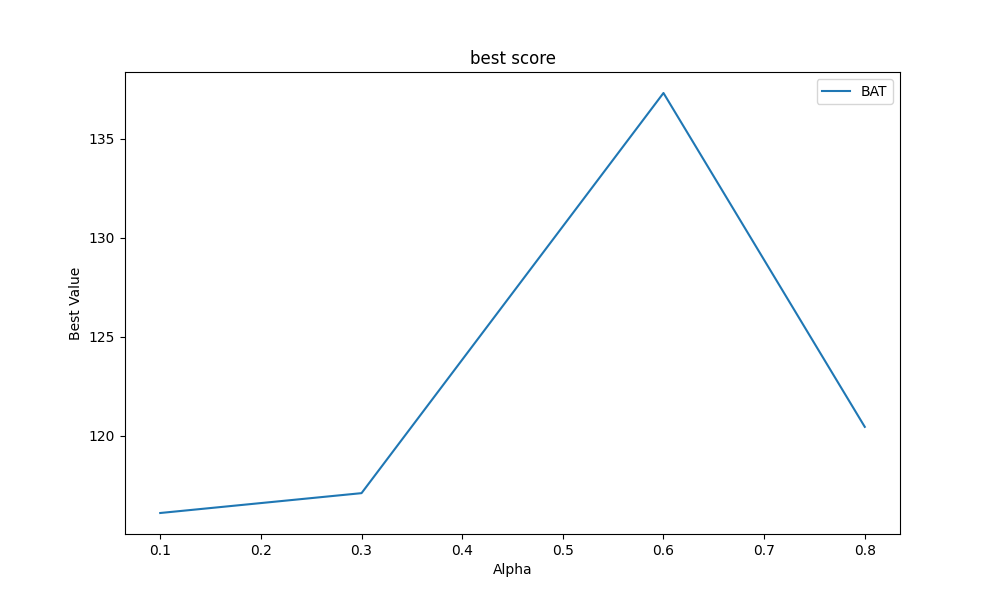
\includegraphics[width=1\textwidth]{plots/bat_alpha.png}
\caption{Wynik eksperymentu dla parametru $\alpha$ dla algorytmu nietoperza.}
\label{fig:alpha_bat}
\end{figure}

\subsection{Wpływ parametru $\epsilon$ dla algorytmu nietoperza}

\begin{figure}[H]
\centering
\includegraphics[width=1\textwidth]{plots/bat_epsilon.png}
\caption{Wynik eksperymentu dla parametru $\epsilon$ dla algorytmu nietoperza.}
\label{fig:epsilon_bat}
\end{figure}

\subsection{Wpływ parametru $\alpha$ dla algorytmu BOA z lotem Levy’ego}

\begin{figure}[H]
\centering
\includegraphics[width=1\textwidth]{plots/boa_levy_alpha.png}
\caption{Wynik eksperymentu dla parametru $\alpha$ dla algorytmu BOA z lotem Levy’ego.}
\label{fig:alpha_levy}
\end{figure}
